\begin{figure*}[h!]
	\begin{subfigure}{\linewidth}
		\caption{}
		\centering
		% include first image
		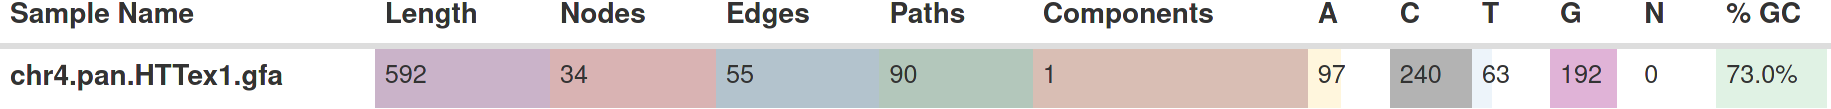
\includegraphics[width=1.0\linewidth]{fig/metrics/chr4.pan.HTTex1.gfa.multiqc_odgi_stats.png}  
		\label{fig:metrics-multiqc}
	\end{subfigure}

	\begin{subfigure}{.5\linewidth}
		\caption{}
		\centering
		% include second image
		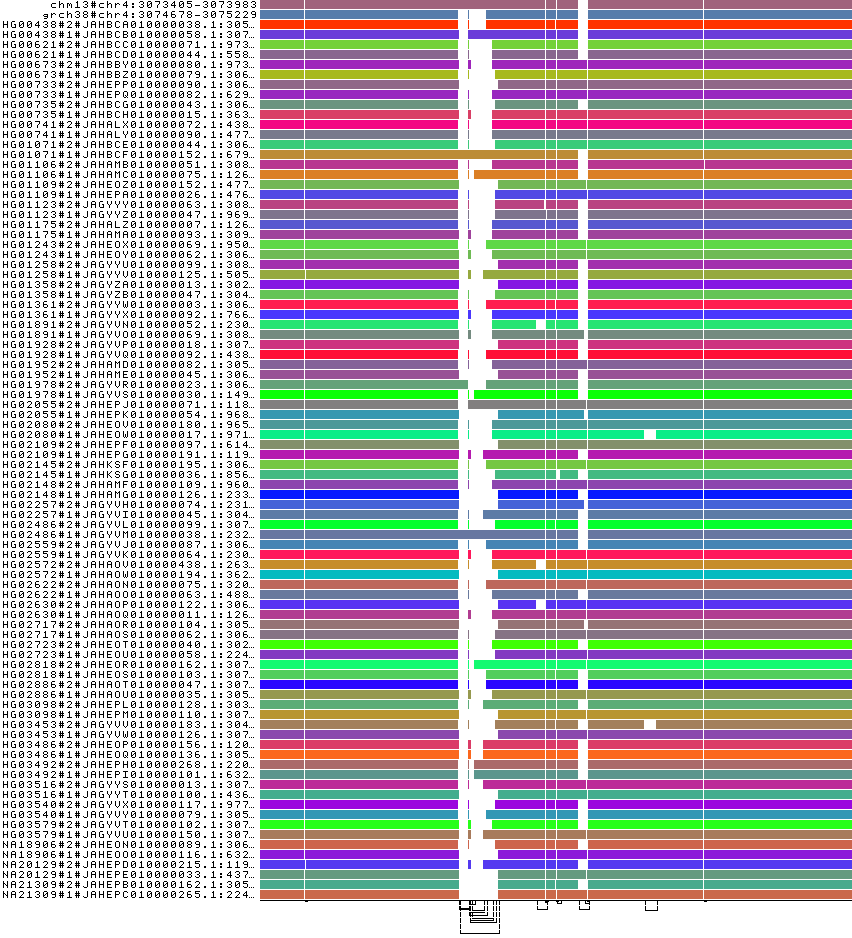
\includegraphics[width=1.0\linewidth]{fig/metrics/chr4.pan.fa.a2fb268.e820cd3.9ea71d8.smooth.gfa.og.HTTex1.og.O.og.png}  
		\label{fig:metrics-viz}
	\end{subfigure}
	\begin{subfigure}{.5\linewidth}
		\caption{}
		\centering
		% include second image
		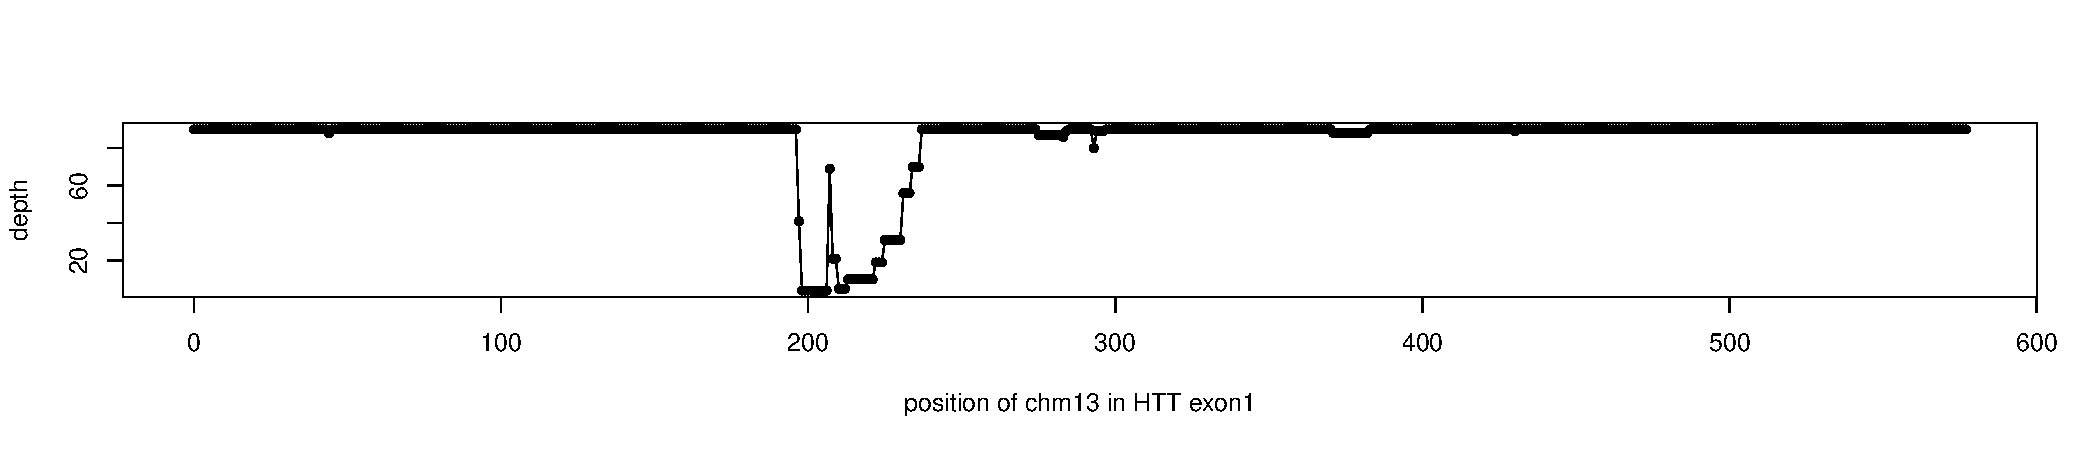
\includegraphics[width=1.0\linewidth]{fig/metrics/chr4.HTT.chm13.depth.w1.bed.pdf}  
		\label{fig:metrics-depth}
	\end{subfigure}

	\begin{subfigure}{.5\linewidth}
		\caption{}
		\centering
		% include third image
		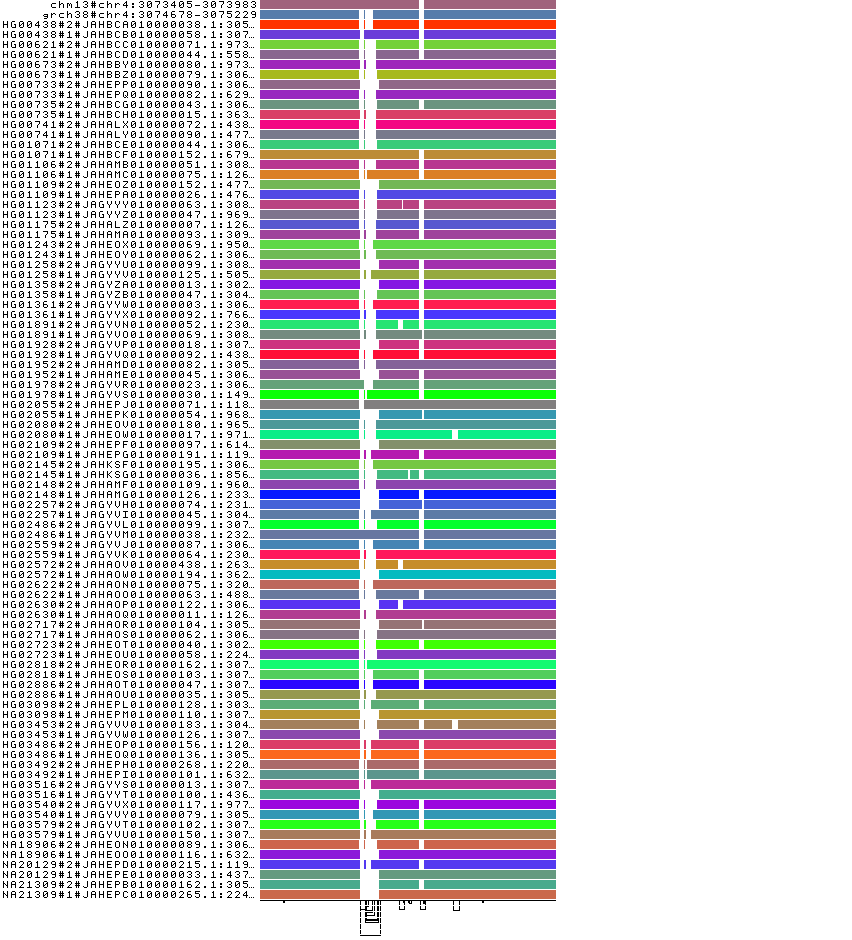
\includegraphics[width=1.0\linewidth]{fig/metrics/chr4.pan.fa.a2fb268.e820cd3.9ea71d8.smooth.gfa.og.HTTex1.og.O.og.w2.convert.png}  
		\label{fig:metrics-bin}
	\end{subfigure}
	\begin{subfigure}{.5\linewidth}
		\caption{}
		\centering
		% include fourth image
		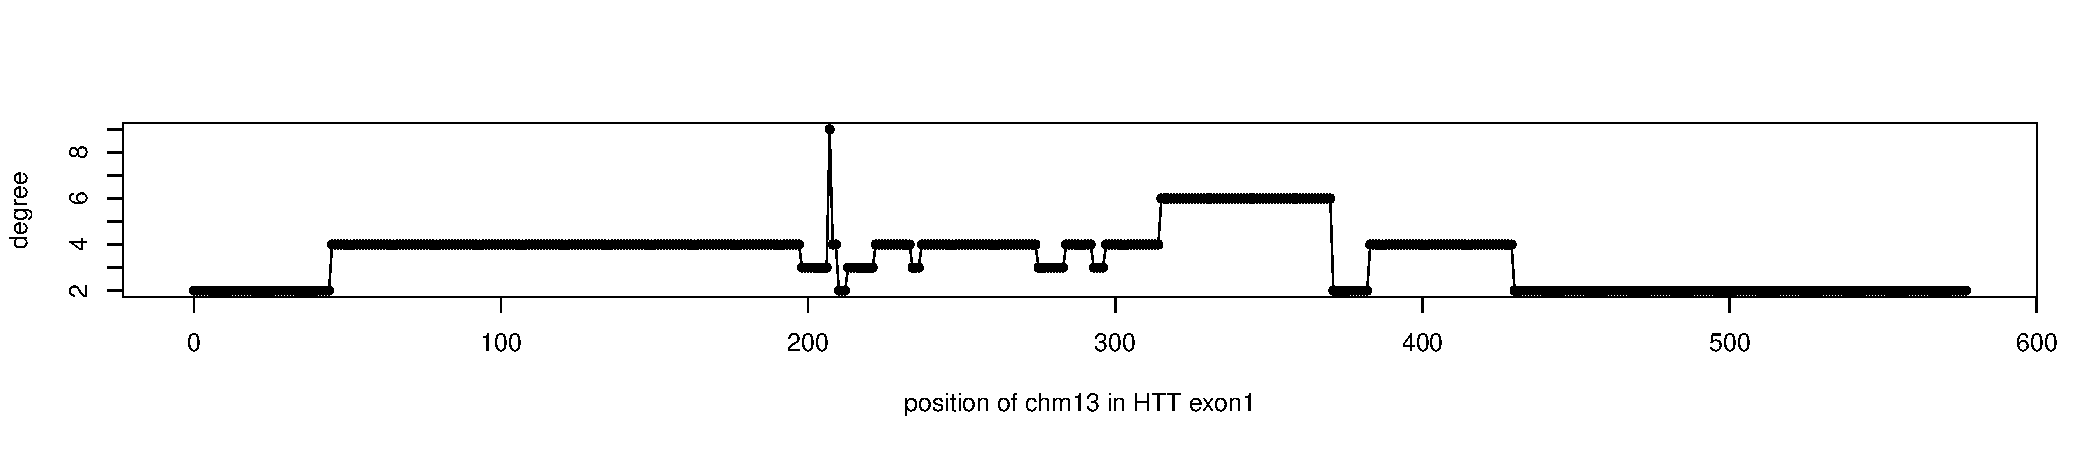
\includegraphics[width=1.0\linewidth]{fig/metrics/chr4.HTT.chm13.degree.w1.bed.pdf}  
		\label{fig:metrics-degree}
	\end{subfigure}
%	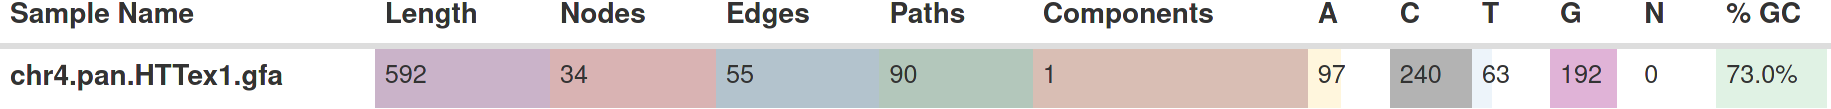
\includegraphics[width=\linewidth]{fig/metrics/chr4.pan.HTTex1.gfa.multiqc_odgi_stats.png}
	\caption{Features of a human pangenome graph of the exon 1 huntingtin gene (\textit{HTTexon1}): \textbf{(a)} Excerpt of vital statistics of the \textit{HTTexon1} graph displayed by MultiQC's ODGI module. The very high GC content of 73.0\% compared to a human genomic mean GC content of 40.9\% \cite{Piovesan2019} is in accordance with the literature (see for example \cite{Sathasivam2013, Neueder2017}). \textbf{(b)} 1D visualization of the \textit{HTTexon1} graph with a bin width of 1. \textbf{(c)} Per nucleotide node depth distribution of CHM13 in the \textit{HTTexon1} graph. The alternating depth around position 200 indicates polymorphic variation. \textbf{(d)} 1D visualization of the \textit{HTTexon1} graph with a bin width of 2. Compared to above, the graph's width is exactly one half, therefore small variation is not visible anymore and the resolution of graph topology decreases. \textbf{(e)} Per nucleotide node degree distribution of CHM13 in the \textit{HTTexon1} graph. The polymorphic region is around position 200 complementing the above node depth analysis. Figures \textbf{(b)-(e)} clearly highlight the variant region around position 200.}
	\label{fig:metrics}
\end{figure*}